\documentclass[12pt]{article}

\usepackage{main}

% TikZ
\usepackage{tikz}

\title{\textbf{Exemples de l'utilisation de TikZ} \\
		La version de TikZ est : \pgfversion}
\author{Régis Santet}
\date{\today}

\begin{document}
	
	\maketitle
	
	\newpage
	\tableofcontents
	\newpage
	
\section{Premières figures}
	
		\subsection{Théorème de Thalès}
			
			\begin{center}
				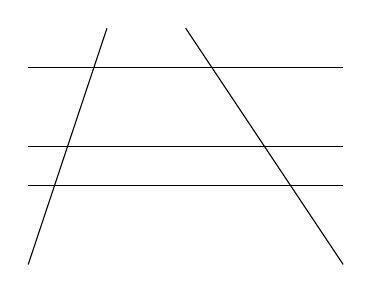
\begin{tikzpicture}
				\draw (0,0) -- (1,3);
				\draw (4,0) -- (2,3);
				
				\draw (0,1) -- (4,1);
				\draw (0,1.5) -- (4, 1.5);
				\draw (0, 2.5) -- (4, 2.5);
				\end{tikzpicture}
			\end{center}
		
		\subsection{Parallélogramme}
			
			\begin{center}
				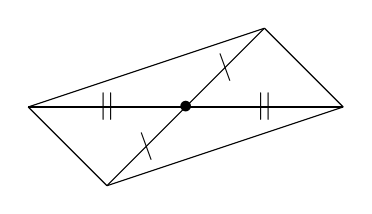
\begin{tikzpicture}
				\draw (0,0) node {$\bullet$};
				\draw (-2,0) -- (2,0);
				\draw (1,1) -- (-1,-1);
				\draw (-1,0) node {$||$};
				\draw (1,0) node {$||$};
				\draw (-0.5, -0.5) node {$\backslash$};
				\draw (0.5, 0.5) node {$\backslash$};
				
				\draw (-2,0) -- (-1,-1);
				\draw (2,0) -- (1,1);
				\draw (-2,0) -- (1,1);
				\draw (2,0) -- (-1,-1);
				\end{tikzpicture}
			\end{center}
		
		\subsection{Losange}
			
			\begin{center}
				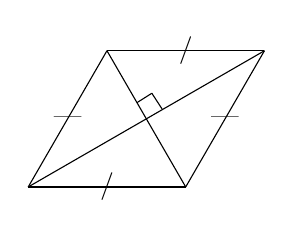
\begin{tikzpicture}
				\draw (0,0) -- (2,0);
				\draw (2,0) -- (3, 1.73);
				\draw (3, 1.73) -- (1, 1.73);
				\draw (0,0) -- (1,1.73);
				
				\draw (0,0) -- (3,1.73);
				\draw (2,0) -- (1, 1.73);
				
				\draw (2, 1.73) node {$/$};
				\draw (1,0) node {$/$};
				
				\draw (2.5, 0.87) node {---};
				\draw (0.5, 0.87) node {---};
				
				\draw (1.38, 1.07) -- (1.57, 1.19);
				\draw (1.57, 1.19) -- (1.7, 0.99);
				\end{tikzpicture}
			\end{center}
			
		\subsection{Centre de gravité}
			
			\begin{center}
				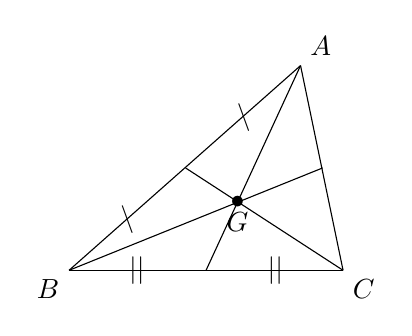
\begin{tikzpicture}[scale=2]
				\draw (0.6, 0.8) -- (-0.87, -0.5);
				\draw (-0.87, -0.5) -- (0.87, -0.5);
				\draw (0.87, -0.5) -- (0.6, 0.8);
				
				\draw (0.6, 0.8) node[above right] {$A$};
				\draw (-0.87, -0.5) node[below left] {$B$};
				\draw (0.87, -0.5) node[below right] {$C$};
				
				\draw (-0.87, -0.5) -- (0.74, 0.15);
				\draw (0.6, 0.8) -- (0, -0.5);
				\draw (0.87, -0.5) -- (-0.13, 0.15);
				
				\draw (0.2, -0.07) node {$\bullet$};
				\draw (0.2, -0.07) node[below] {$G$};
				
				\draw (0.24, 0.47) node {$\backslash$};
				\draw (-0.5, -0.18) node {$\backslash$};
				
				\draw (-0.44, -0.5) node {$||$};
				\draw (0.44, -0.5) node {$||$};
				\end{tikzpicture}
			\end{center}
		
		\subsection{Cerce circonscrit}
			
			\begin{center}
				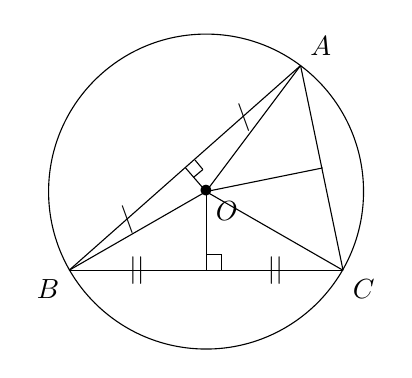
\begin{tikzpicture}[scale=2]
				\draw (0.6, 0.8) -- (-0.87, -0.5);
				\draw (-0.87, -0.5) -- (0.87, -0.5);
				\draw (0.87, -0.5) -- (0.6, 0.8);
				
				\draw (0.6, 0.8) node[above right] {$A$};
				\draw (-0.87, -0.5) node[below left] {$B$};
				\draw (0.87, -0.5) node[below right] {$C$};
				
				\draw (0,0) circle (1);
				\draw (0,0) node[below right] {$O$};
				\draw (0,0) node {$\bullet$};
				
				\draw (-0.87, -0.5) -- (0,0);
				\draw (0.6, 0.8) -- (0,0);
				\draw (0.87, -0.5) -- (0,0);
				
				\draw (0, -0.5) -- (0,0);
				\draw (-0.13, 0.15) -- (0,0);
				\draw (0.74, 0.15) -- (0,0);
				
				\draw (0.1, -0.5) -- (0.1, -0.4);
				\draw (0.1, -0.4) -- (0, -0.4);
				
				\draw (-0.08, 0.09) -- (-0.02, 0.14);
				\draw (-0.02, 0.14) -- (-0.07, 0.2);
				
				\draw (0.24, 0.47) node {$\backslash$};
				\draw (-0.5, -0.18) node {$\backslash$};
				
				\draw (-0.44, -0.5) node {$||$};
				\draw (0.44, -0.5) node {$||$};
				\end{tikzpicture}
			\end{center}
		
		\subsection{Orthocentre}
			
			\begin{center}
				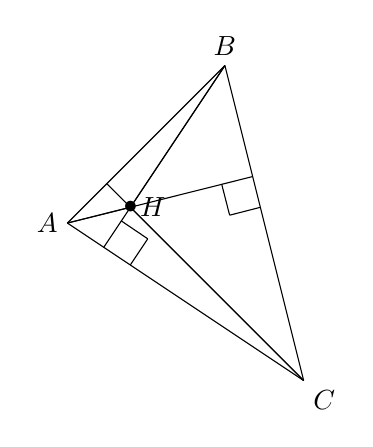
\begin{tikzpicture}
				\draw (0,0) node[left] {$A$};
				\draw (2,2) node[above] {$B$};
				\draw (3, -2) node[below right] {$C$};
				
				\draw (0,0) -- (2,2);
				\draw (2,2) -- (3,-2);
				\draw (3,-2) -- (0,0);
				
				\draw (0.8, 0.2) node {$\bullet$};
				\draw (0.8, 0.2) node[right] {$H$};
				
				\draw (0,0) -- (0.8, 0.2);
				\draw (2,2) -- (0.8, 0.2);
				\draw (3, -2) -- (0.8, 0.2);
				
				\draw (0.46, -0.31) -- (2,2);
				\draw (2.35, 0.59) -- (0,0);
				\draw (0.5, 0.5) -- (3, -2);
				
				\draw (0.8, -0.53) -- (1.02, -0.2);
				\draw (1.02, -0.2) -- (0.68, 0.03);
				
				\draw (1.96, 0.49) -- (2.06, 0.1);
				\draw (2.06, 0.1) -- (2.45, 0.2);
				\end{tikzpicture}
			\end{center}
			
		\subsection{Centre du cercle inscrit}
			
			\begin{center}
				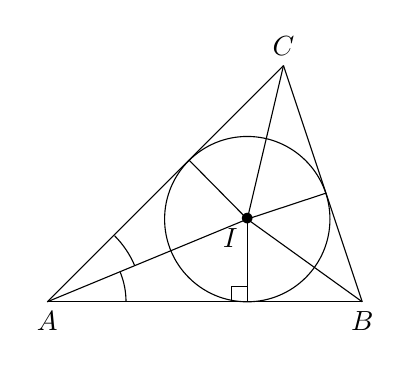
\begin{tikzpicture}
				\draw (0,0) node[below] {$A$};
				\draw (4,0) node[below] {$B$};
				\draw (3,3) node[above] {$C$};
				
				\draw (0,0) -- (4,0);
				\draw (4,0) -- (3,3);
				\draw (3,3) -- (0,0);
				
				\draw (2.54, 1.05) circle (1.05);
				\draw (2.54, 1.05) node[below left] {$I$};
				\draw (2.54, 1.05) node {$\bullet$};
				
				\draw (2.54, 0) -- (2.54, 1.05);
				\draw (1.8, 1.8) -- (2.54, 1.05);
				\draw (3.54, 1.38) -- (2.54, 1.05);
				
				\draw (0,0) -- (2.54, 1.05);
				\draw (4,0) -- (2.54, 1.05);
				\draw (3,3) -- (2.54, 1.05);
				
				\draw (2.34, 0) -- (2.34, 0.2);
				\draw (2.34, 0.2) -- (2.54, 0.2);
				
				\draw (1,0) arc (0:22:1);
				\draw (1.11, 0.46) arc (23:45:1.2);
				\end{tikzpicture}
			\end{center}
		
\section{Chemins, options graphiques}
	
	\subsection{Somme de deux vecteurs}
	\tikzstyle{vecteur}=[->, >=stealth]
	\begin{center}
		\begin{tikzpicture}[scale=3]
		\draw[vecteur] (0,0) -- (0.5,1) node[above] {$\vec{u}$};
		\draw[vecteur] (0,0) -- (1, 0) node[below right] {$\vec{v}$};
		\draw[vecteur] (0,0) -- (1.5, 1) node[below right] {$\vec{u}+\vec{v}$};
		
		\draw[dashed] (1,0) -- (1.5, 1);
		\draw[dashed] (0.5,1) -- (1.5,1);
		\end{tikzpicture}
		
		\begin{tikzpicture}[scale=3]
		\draw[vecteur] (0,0) -- (0.5,1) node[midway, left] {$\vec{u}$};
		\draw[vecteur] (0,0) -- (1.5,1) node[midway, below right] {$\vec{u}+\vec{v}$};
		\draw (0.5,1) -- (1.5,1) node[midway, above] {$\vec{v}$};
		\end{tikzpicture}
	\end{center}

	\subsection{Triangle rectangle inscrit dans un demi-cercle}
	
	\begin{center}
		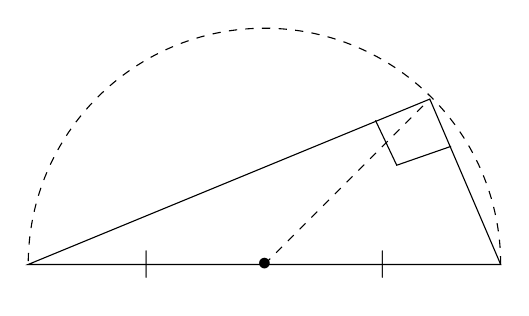
\begin{tikzpicture}[scale=3]
		\draw (0,0) node {$\bullet$};
		\draw (-1,0) -- (1,0) -- (0.7, 0.7) -- cycle;
		\draw (-0.5, 0) node {$|$};
		\draw (0.5, 0) node {$|$};
		
		\draw[dashed] (0,0) -- (0.7, 0.7);
		\draw[dashed] (1,0) arc (0:180:1);
		
		\draw (0.79, 0.5) -- (0.56, 0.42) -- (0.47, 0.61);
		\end{tikzpicture}
	\end{center}

	\subsection{Angle inscrit et angle au centre}
	
	\begin{center}
		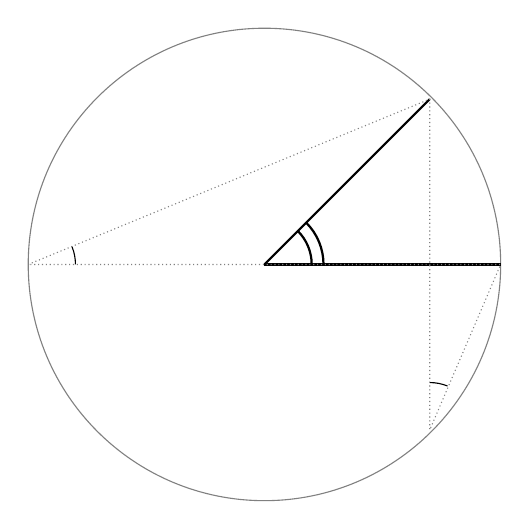
\begin{tikzpicture}[scale=3]
		\draw[color=gray] (0,0) circle (1);
		\draw[thick] (0,0) -- (1,0);
		\draw[thick] (0,0) -- (0.7, 0.7);
		\draw[thick] (0.2,0) arc (0:45:0.2);
		\draw[thick] (0.25,0) arc (0:45:0.25);
		
		\draw[densely dotted, color=gray] (-1,0) -- (0.7,0.7) -- (0.7, -0.7) -- (1,0) -- cycle;
		
		\draw (-0.8,0) arc (0:22:0.2);
		\draw (0.7, -0.5) arc (90:68:0.2);
		\end{tikzpicture}
	\end{center}

	\subsection{Parallèles, aires égales}
	
	\begin{center}
		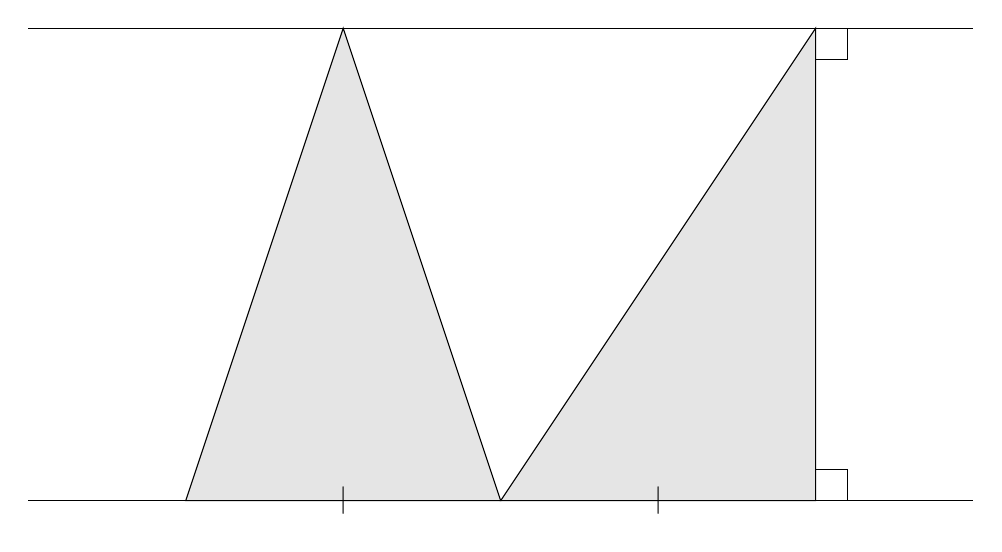
\begin{tikzpicture}[scale=2]
		\draw (-3,0) -- (3,0);
		\draw (-3,3) -- (3,3);
		
		\draw[fill=gray!20] (-2,0) -- (-1,3) -- (0,0) -- cycle;
		\draw[fill=gray!20] (0,0) -- (2,3) -- (2,0) -- cycle;
		
		\draw (-1,0) node {$|$};
		\draw (1,0) node {$|$};
		
		\draw (2.2, 0) -- (2.2, 0.2) -- (2, 0.2);
		\draw (2.2, 3) -- (2.2, 2.8) -- (2, 2.8);		
		\end{tikzpicture}
	\end{center}

	\subsection{Composée de deux symétries centrales}
	
	\begin{center}
		\begin{tikzpicture}[scale=3]
		\draw (0,0) -- (0.5,1) node[midway] {$-$};
		\draw (0.5,1) -- (1,2) node[midway] {$-$};
		\draw (0,0) -- (1, 0.5) node[midway] {$||$};
		\draw (1, 0.5) -- (2,1) node[midway] {$||$};
		
		\draw (0,0) node[below] {$M_1$};
		\draw (0.5,1) node[left] {$I_1$} node {$\bullet$};
		\draw (1,0.5) node[below right] {$I_2$} node {$\bullet$};
		\draw (1,2) node[above] {$M$};
		\draw (2,1) node[right] {$M_2$};
		
		\draw[->, >=latex, dashed] (1,2) -- (2,1) node[midway, above] {$2\vec{v}$};
		\draw[->, >=latex, dashed] (0.5,1) -- (1,0.5) node[midway, above] {$\vec{v}$}; 
		\end{tikzpicture}
	\end{center}
	
	\subsection{Suite géométrique}
	
	\begin{center}
		\begin{tikzpicture}[scale=5]
		\draw (0,0) -- (1,0) -- (0.5, 0.5) -- cycle;
		\draw (0,0) node[left] {$O$};
		\draw (1,0) node[right] {$A$};
		\draw (0.5, 0.5) node[above] {$B$};
		
		\draw (0.5,0.5) -- (0.5,0) -- (0.75, 0.25) -- (0.75, 0) -- (0.87, 0.13) -- (0.87, 0) -- (0.94, 0.06) -- (0.94, 0) -- (0.97, 0.03) -- (0.97, 0);
		
		\draw[dashed] (0,0) -- (0,-0.65);
		\draw[dashed] (1,0) -- (1,-0.65);
		\draw[dashed] (0.5,0) -- (0.5,-0.25);
		\draw[dashed] (0.75,0) -- (0.75,-0.25);
		\draw[dashed] (0.87,0) -- (0.87, -0.25);
		
		\draw[<->, >=latex] (0,-0.65) -- (1,-0.65) node[midway, below] {$1$};
		\draw[<->, >=latex] (0,-0.25) -- (0.5, -0.25) node[midway, below] {$\dfrac{1}{2}$};
		\draw[<->, >=latex] (0.5,-0.25) -- (0.75, -0.25) node[midway, below] {$\dfrac{1}{4}$};
		\draw[<->, >=latex] (0.75,-0.25) -- (0.87, -0.25) node[midway, below] {$\dfrac{1}{8}$};
		\end{tikzpicture}
	\end{center}
	
\section{Courbes}
	
	\subsection{Ellipse. Angles avec \texttt{circle} et \texttt{\\clip}}
	
	\begin{center}
		\begin{tikzpicture}
		\draw[samples=200] plot ({5*cos(\x r)}, {3*sin(\x r)});
		
		\coordinate (F1) at (-4, 0);
		\coordinate (F2) at (4, 0);
		\coordinate (A) at (2,2.75);
		\coordinate (P) at (1.28, 0);
		\draw (F1) node {$\bullet$} node[below] {$F'$};
		\draw (F2) node {$\bullet$} node[below] {$F$};
		\draw (A) node[above right] {$A$};
		
		\draw[->] (-6,0) -- (6,0);
		\draw[->] (0,-5) -- (0,5);
		\draw (F1) -- (F2) -- (A) -- cycle;
		\draw (2.25, 3.72) -- (1.28, 3.97) -- (1.03, 3);
		
		\draw[dashed] plot [domain=-3:5] (\x, {-0.26*\x+3.27});
		\draw[dashed] plot [domain=1:2.5] (\x, {3.82*\x-4.89});
		
		\draw[color=gray] (P) node[below right] {$P$};
		
		\begin{scope}
		\clip (A) -- (P) -- (F2) -- cycle;
		\draw[color=gray] (A) circle (1.2);
		\end{scope}
		
		\begin{scope}
		\clip (F1) -- (A) -- (P) -- cycle;
		\draw[color=gray] (A) circle (1);
		\end{scope}
		\end{tikzpicture}
	\end{center}

	\subsection{$a^b = b^a$. \texttt{xscale, yscale}}
	
	\begin{center}
		\begin{tikzpicture}
		\draw (0,0) node [below right] {$0$};
		\draw (1,0) node [below right] {$1$};
		\draw (2,0) node [below right] {$2$};
		\draw (3,0) node [below right] {$3$};
		
		\draw[samples=50] plot [domain=0.5:6] (\x, {ln(\x)/\x});
		\draw[dashed] ({exp(1)},0) -- ({exp(1)}, {exp(-1)});
		\draw ({exp(1)},0) node [below] {$e$};
		\draw (-2, 0) -- (6,0);
		\draw (0,-2) -- (0,2);
		\end{tikzpicture}
	\end{center}

	\subsection{Fonction périodique : \texttt{$\backslash$foreach}}
	
	\begin{center}
		\begin{tikzpicture} [domain=-1:1, samples=80]
		\foreach \k in {0,2,...,8}
			{\draw plot (\x + \k, \x^3);}
		\end{tikzpicture}
	\end{center}

	\subsection{Fonctions réciproques, aires : \texttt{pattern}}
	
	\begin{center}
		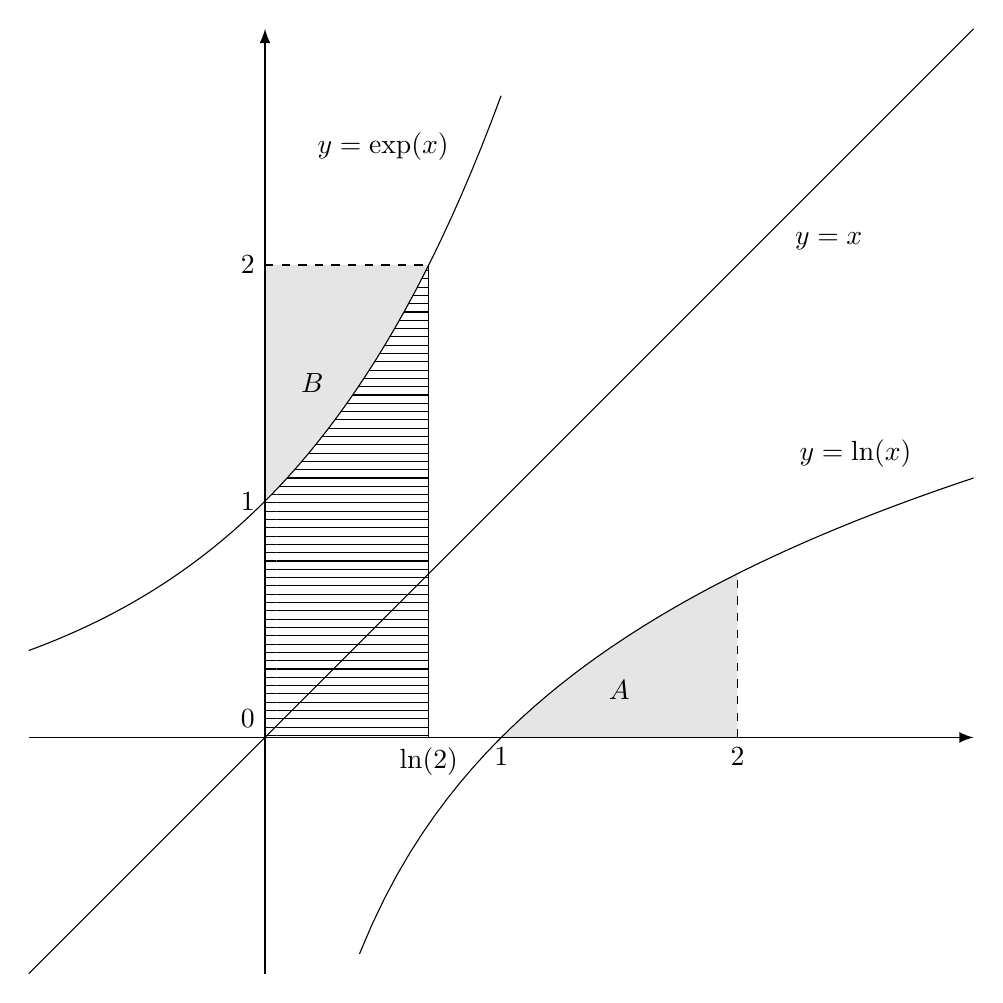
\begin{tikzpicture}[scale=3]
		\usetikzlibrary{patterns}
		\fill [pattern=horizontal lines]
		(0,0)
		-- plot [domain=0:{ln(2)}] (\x, {exp(\x)})
		-- ({ln(2)}, 0)
		-- cycle;
		
		\fill [color=gray!20]
		plot [domain=0:{ln(2)}] (\x, {exp(\x)})
		-- ({ln(2)},2) -- (0,2) -- cycle;
		\fill [color=gray!20]
		plot [domain=1:2] (\x, {ln(\x)})
		 -- (2,0) -- (1,0) -- cycle;
		 \draw [dashed] (0,2) -- ({ln(2)},2);
		 \draw [dashed] (2,0) -- (2, {ln(2)});
		 \draw ({ln(2)},0) -- ({ln(2)},2);
		
		\draw[->, >=latex] (-1,0) -- (3,0);
		\draw[->, >=latex] (0,-1) -- (0,3);
		\draw (0,0) node [above left] {$0$};
		\draw (1,0) node [below] {$1$};
		\draw (2,0) node [below] {$2$};
		\draw ({ln(2)},0) node [below] {$\ln(2)$};
		\draw (0,1) node [left] {$1$};
		\draw (0,2) node [left] {$2$};
		
		\draw plot [domain=-1:1, samples=50] (\x, {exp(\x)});
		\draw plot [domain=0.4:3, samples=50] (\x, {ln(\x)});
		\draw plot [domain=-1:3, samples=50] (\x, \x);
		
		\draw (0.2, 1.5) node {$B$};
		\draw (1.5, 0.2) node {$A$};
		
		\draw (0.5, 2.5) node {$y=\exp(x)$};
		\draw (2.5, 1.2) node {$y=\ln(x)$};
		\draw (2.2, 2.1) node [right] {$y=x$};
		
		\end{tikzpicture}
	\end{center}

	\subsection{Lemniscate de Gerono. \texttt{$\backslash$scope, xshift, $\backslash$filldraw}}
	
	\begin{center}
		\begin{tikzpicture}[scale=2]
		\begin{scope}
		\filldraw[fill=gray!20] plot[samples=50, domain=-pi:pi] ({cos(\x r)}, {cos(\x r)*sin(\x r)});
		\draw (0,-1) node {$A$}; 
		\end{scope}
		
		\begin{scope}[xshift=2.3cm]
		\draw [dashed] plot[samples=50, domain={-pi}:{pi}] ({cos(\x r)},{sin(\x r)*cos(\x r)});
		\filldraw[fill=gray!20] ({-sqrt(2)/2}, -0.5) -- ({sqrt(2)/2}, 0.5) -- (1, 0) -- ({sqrt(2)/2}, -0.5) -- ({-sqrt(2)/2}, 0.5) -- (-1,0) -- cycle;
		\draw (0,-1) node {$1 \leq A$}; 
		\end{scope}
		
		\begin{scope}[xshift=4.6cm]
		\filldraw [fill=gray!20] (-1,-0.5) -- (-1, 0.5) -- (-0.5, 0.5) -- (0.5, -0.5) -- (1, -0.5) -- (1, 0.5) -- (0.5, 0.5) -- (-0.5, -0.5) -- cycle;
		\draw [dashed] plot[samples=50, domain={-pi}:{pi}] ({cos(\x r)},{sin(\x r)*cos(\x r)});
		\draw (0,-1) node {$A \leq \dfrac{3}{2}$}; 
		\end{scope}
		
		\begin{scope}[xshift=6.9cm]
		\draw (0,0) node {\fbox{$1 \leq A \leq \dfrac{3}{2}$}};
		\end{scope}
		\end{tikzpicture}
	\end{center}

\section{Géométrie dans l'espace}
	% Leur <-> Mien
	% x <-> z
	% y <-> x
	% z <-> y
	\subsection{Section d'un cube suivant un hexagone}
	
	\begin{center}
		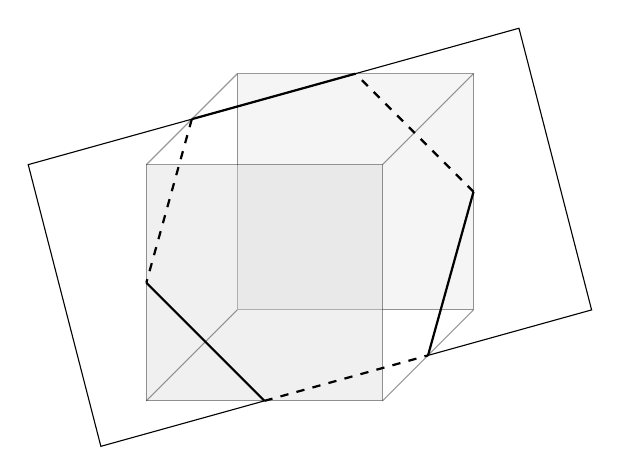
\begin{tikzpicture}[scale=3]
		
		\filldraw [fill=gray!20, opacity=0.4] (0,0,0) -- (1,0,0) -- (1,1,0) -- (0,1,0) -- cycle;
		\filldraw [fill=gray!30, opacity=0.4] (0,0,1) -- (1,0,1) -- (1,1,1) -- (0,1,1) -- cycle;
		\draw[opacity=0.4] (0,0,0) -- (0,0,1);
		\draw[opacity=0.4] (1,0,0) -- (1,0,1);
		\draw[opacity=0.4] (1,1,0) -- (1,1,1);
		\draw[opacity=0.4] (0,1,0) -- (0,1,1);
		
		\draw (0.5, 0, 1) -- (0,0,3/2) -- (-0.5,1,1) -- (1, 1, -0.5) -- (3/2, 0, 0) -- (1, 0, 0.5);
		
		\draw[thick, dashed] (0.5, 0, 1) -- (1, 0, 0.5);
		\draw[thick, dashed] (1, 0.5, 0) -- (0.5, 1, 0);
		\draw[thick, dashed] (0, 1, 0.5) -- (0, 0.5, 1);
		\draw[thick] (0.5, 0, 1) -- (0, 0.5, 1);
		\draw[thick] (1, 0, 0.5) -- (1, 0.5, 0);
		\draw[thick] (0, 1, 0.5) -- (0.5, 1, 0);
		
	
		\end{tikzpicture}
	\end{center}

	\subsection{Grande diagonale d'un cube}
	
	\begin{center}
		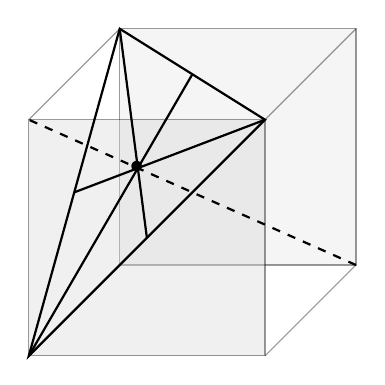
\begin{tikzpicture}[scale=3]
		\filldraw [fill=gray!20, opacity=0.4] (0,0,0) -- (1,0,0) -- (1,1,0) -- (0,1,0) -- cycle;
		\filldraw [fill=gray!30, opacity=0.4] (0,0,1) -- (1,0,1) -- (1,1,1) -- (0,1,1) -- cycle;
		\draw[opacity=0.4] (0,0,0) -- (0,0,1);
		\draw[opacity=0.4] (1,0,0) -- (1,0,1);
		\draw[opacity=0.4] (1,1,0) -- (1,1,1);
		\draw[opacity=0.4] (0,1,0) -- (0,1,1);
		
		% Grande diagonale
		\draw[dashed, thick] (1,0,0) -- (0,1,1);
		
		% Triangle équilatéral
		\draw[thick] (0,1,0) -- (1,1,1) -- (0, 0, 1) -- cycle;
		\draw[thick] (0, 0.5, 0.5) -- (1,1,1);
		\draw[thick] (0.5, 0.5, 1) -- (0,1,0);
		\draw[thick] (0.5, 1, 0.5) -- (0,0,1);
		
		\draw (0.33, 0.67, 0.67) node {$\bullet$};
		\end{tikzpicture}
	\end{center}

	\subsection{Droites et plans}
	
	\begin{center}
		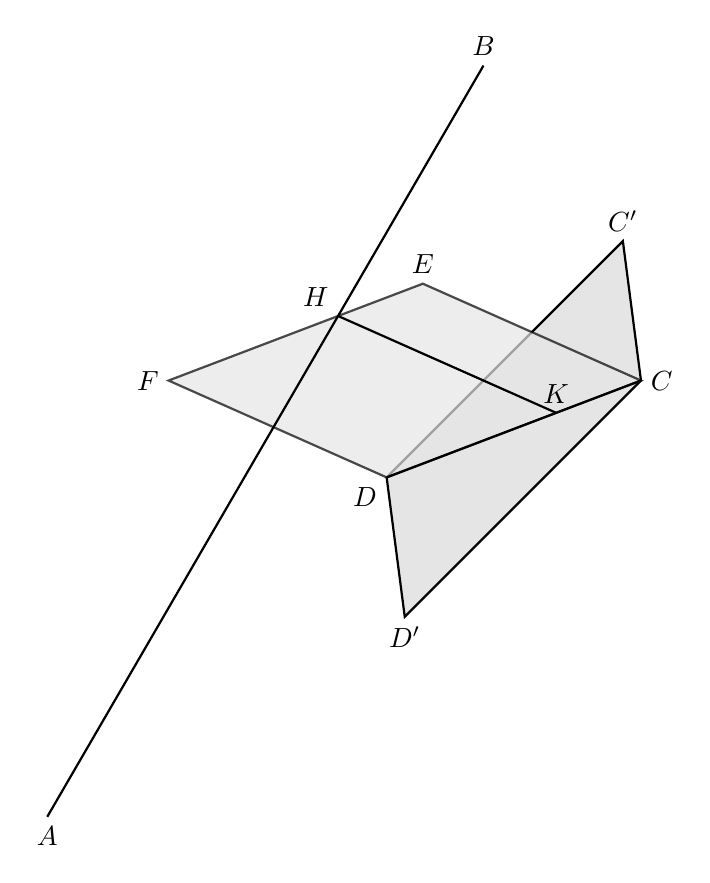
\begin{tikzpicture}[scale=2]
		\coordinate (A) at (-1, -2, 2);
		\coordinate (B) at (1, 2, 0);
		\coordinate (C) at (2, 0, 0);
		\coordinate (D) at (0, -1, -1);
		\coordinate (Cprime) at (3/2, 1/2, -1);
		\coordinate (Dprime) at (1/2, -3/2, 0);
		\coordinate (E) at (1,1,1);
		\coordinate (F) at (-1,0,0);
		\coordinate (H) at (1/3, 2/3, 2/3);
		\coordinate (K) at (4/3, -1/3, -1/3);
		
		
		\filldraw[thick, fill=gray!20] (D) -- (Cprime) -- (C) -- (Dprime) -- cycle;
		\filldraw[thick, fill=gray!20, opacity=0.7] (F) -- (E) -- (C) -- (D) -- cycle;
		\draw[thick] (A) -- (B); \draw[thick] (C) -- (D);
		\draw[thick] (K) -- (H);
		
		\draw (A) node[below] {$A$};
		\draw (B) node[above] {$B$};
		\draw (C) node[right] {$C$};
		\draw (Cprime) node[above] {$C'$};
		\draw (D) node[below left] {$D$};
		\draw (Dprime) node[below] {$D'$};
		\draw (E) node[above] {$E$};
		\draw (F) node[left] {$F$};
		\draw (K) node[above] {$K$};
		\draw (H) node[above left] {$H$};
		\end{tikzpicture}
	\end{center}

	\subsection{Courbes et surfaces}
	\subsubsection{Hélice}
	\begin{center}
		\begin{tikzpicture}[scale=2]
		\draw [domain=-4*pi:4*pi, samples=80, smooth]
		plot ({cos(\x r)},{sin(\x r)}, \x/pi);
		\end{tikzpicture}
	\end{center}

	\subsubsection{Cylindre}
	\begin{center}
		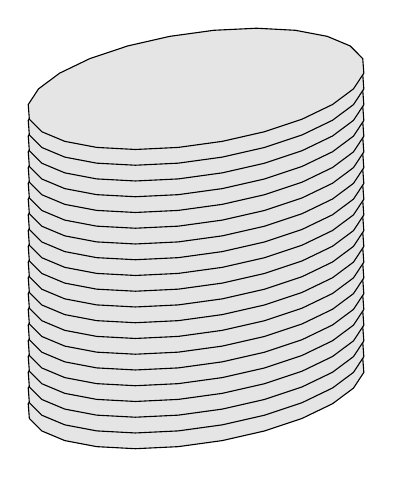
\begin{tikzpicture}[scale=2]
		\foreach \t in {-1,-0.9,...,1} {
			\filldraw[fill=gray!20] plot[domain=0:2*pi]
			({cos(\x r)}, \t, {sin(\x r)});
		}
		\end{tikzpicture}
	\end{center}

	\subsection{Sphère}
	\begin{center}
		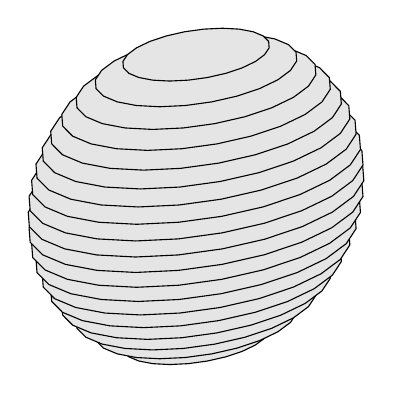
\begin{tikzpicture}[scale=2]
		\foreach \t in {-1,-0.9,...,1} {
			\filldraw[fill=gray!20] plot[domain=0:2*pi]
			({sqrt(1-\t*\t)*cos(\x r)}, \t, {sqrt(1-\t*\t)*sin(\x r)});
		}
		\end{tikzpicture}
	\end{center}

	\subsection{Paraboloïde}
	\begin{center}
		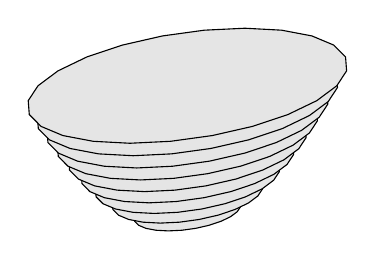
\begin{tikzpicture}[scale=2]
		\foreach \t in {0,0.1,...,1} {
			\filldraw[fill=gray!20] plot[domain=0:2*pi]
			({sqrt(\t)*cos(\x r)}, \t, {sqrt(\t)*sin(\x r)});
		}
		\end{tikzpicture}
	\end{center}

\section{Représentation de données}

\newcommand{\nombresCopiesParNote}
{(0,0)(1,0)(2,2)(3,0)(4,6)(5,4)(6,7)(7,4)(8,3)(9,0)(10,1)}

	\subsection{Notions de base}
	\subsubsection{Diagramme d'effectifs : \texttt{plot coordinates}}

	\begin{center}
		\begin{tikzpicture}
		\draw plot coordinates {(0,0) (1,0) (2,2) (3,0)
			(4,6) (5,4) (6,7) (7,4) (8,3) (9,0) (10,1)};
		%draw plot coordinates {\nombresCopiesParNote}
		\end{tikzpicture}
	\end{center}
	
	
	\subsubsection{Améliorer la lisibilité : \texttt{grid, node, $\backslash$foreach}}
	
	\begin{center}
		\begin{tikzpicture}
		\draw (-1,0) grid (11,7);
		
		\foreach \y in {1,2,...,7} \draw(-1,\y)node[left]{\y};
		\foreach \x in {0,1,...,10} \draw(\x,0)node[below]{\x};
		
		\draw plot coordinates {\nombresCopiesParNote};
		\end{tikzpicture}
	\end{center}

	\subsubsection{Marquer les points, étiqueter : \texttt{mark, node, rotate}}
	
	\begin{center}
		\begin{tikzpicture}
		\draw (-1,0) grid (11,7);
		
		\foreach \y in {1,2,...,7}
		\draw (-1, \y)node[left]{\y};
		\foreach \x in {0,1,...,10}
		\draw (\x,0) node[below]{\x};
		
		\draw (5.5, -0.75) node{Notes};
		\draw (-1.75, 3.5) node[rotate=90]{Nombre de notes};
		
		\draw[thick] plot[mark=*] coordinates {\nombresCopiesParNote};
		\end{tikzpicture}
	\end{center}
	
	\subsubsection{Diagramme à barres : \texttt{xcomb, ycomb, polar comb}}
	
	\begin{center}
		\begin{tikzpicture}
		\draw (-1,0) grid (11,7);
		
		\foreach \y in {1,2,...,7}
		\draw (-1, \y)node[left]{\y};
		\foreach \x in {0,1,...,10}
		\draw (\x,0) node[below]{\x};
		
		\draw (5.5, -0.75) node{Notes};
		\draw (-1.75, 3.5) node[rotate=90]{Nombre de notes};
		
		\draw[thick, line width=4pt] plot[mark=*, ycomb] coordinates {\nombresCopiesParNote};
		\end{tikzpicture}
	\end{center}	

	\subsubsection{Histogramme : \texttt{xcomb, ycomb, line width}}
	
		\begin{center}
		\begin{tikzpicture}
		\draw (-1,0) grid (11,7);
		
		\foreach \y in {1,2,...,7}
		\draw (-1, \y)node[left]{\y};
		\foreach \x in {0,1,...,10}
		\draw (\x,0) node[below]{\x};
		
		\draw (5.5, -0.75) node{Notes};
		\draw (-1.75, 3.5) node[rotate=90]{Nombre de notes};
		
		\draw[thick, line width=8mm,color=blue!50] plot[ycomb] coordinates {\nombresCopiesParNote};
		\end{tikzpicture}
	\end{center}
	
	\subsubsection{Affichage des données d'un fichier : \texttt{plot file}}
	
	\begin{center}
		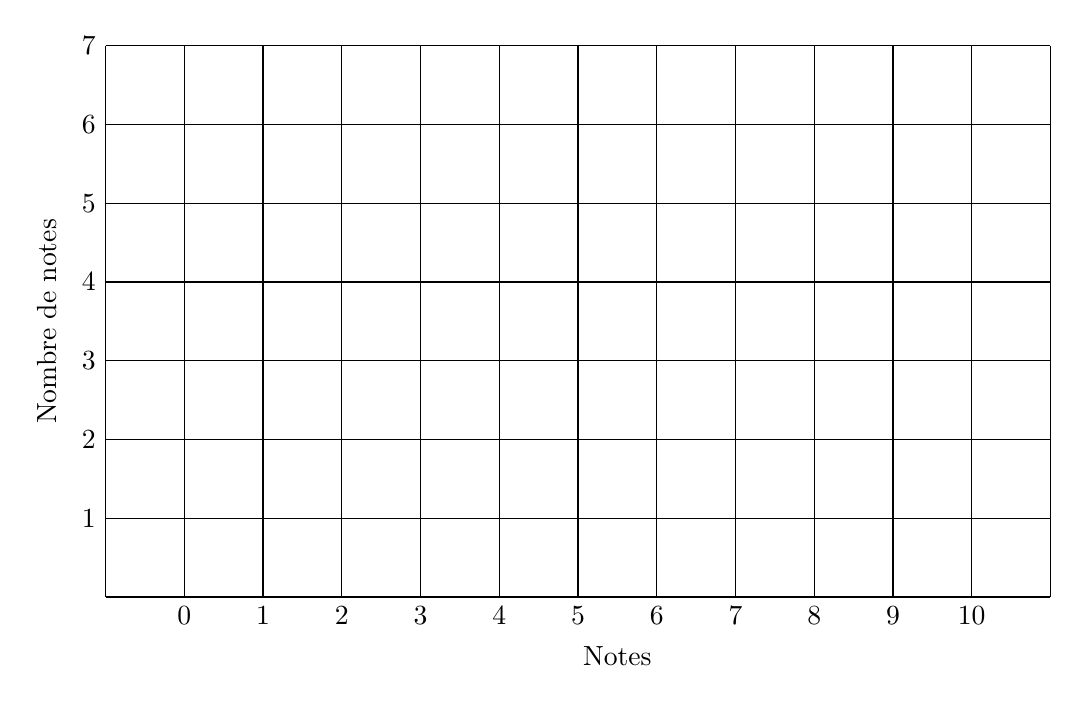
\begin{tikzpicture}
		\draw (-1,0) grid (11,7);
		
		\foreach \y in {1,2,...,7}
		\draw (-1, \y)node[left]{\y};
		\foreach \x in {0,1,...,10}
		\draw (\x,0) node[below]{\x};
		
		\draw (5.5, -0.75) node{Notes};
		\draw (-1.75, 3.5) node[rotate=90]{Nombre de notes};
		
		\draw[thick, line width=8mm, color=blue!50] plot[ycomb] file {nombreCopiesParNote.txt};
		\end{tikzpicture}
	\end{center}

	\subsection{Diagramme à barres horizontales}
	\subsubsection{Barres horizontales : \texttt{plot file, xcomb}}
	
	\begin{center}
		\begin{tikzpicture}[xscale=0.09, yscale=0.6]
		\draw[line width=4mm,color=blue!50]
		plot[xcomb] file {producBle2004.txt};
		\end{tikzpicture}
	\end{center}

	\subsubsection{Installation d'une grille : \texttt{grid, xstep, ystep}}
	
	\begin{center}
		
\begin{tikzpicture}[xscale=0.09, yscale=0.6]
		\draw (0,0) grid[xstep=10,ystep=15] (100,15);
		\draw[gray,very thin] (0,0) grid[xstep=5,ystep=15] (100,15);
		\draw[line width=4mm,color=blue!50]
		plot[xcomb] file {producBle2004.txt};
		\end{tikzpicture}
	\end{center}

	\subsubsection{Etiquetage du repère : \texttt{$\backslash$foreach, node}}

	
	\begin{center}
		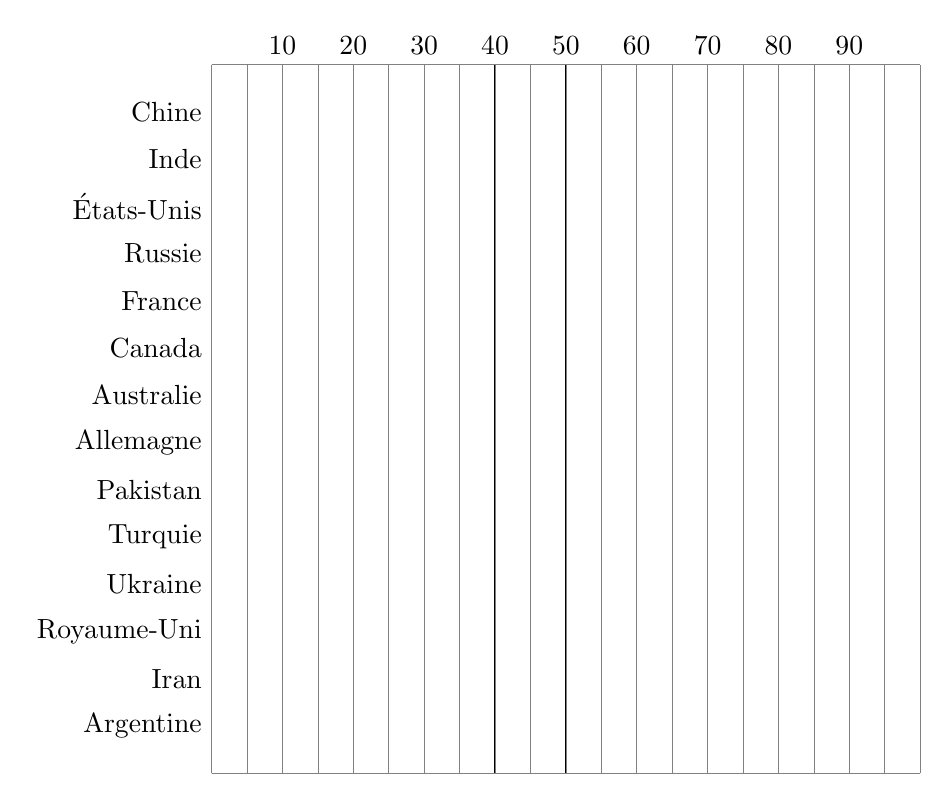
\begin{tikzpicture}[xscale=0.09, yscale=0.6]
		\draw (0,0) grid[xstep=10,ystep=15] (100,15);
		\draw[gray,very thin] (0,0) grid[xstep=5,ystep=15] (100,15);
		\draw[line width=4mm,color=blue!50]
		plot[xcomb] file {producBle2004.txt};
		
		\foreach \x in {10,20,...,90} \draw(\x,15)node[above]{\x};
		\foreach \n/\y in {Chine/14,Inde/13,États-Unis/12,Russie/11,
			France/10,Canada/9,Australie/8,Allemagne/7,Pakistan/6,
			Turquie/5,Ukraine/4,Royaume-Uni/3,Iran/2,Argentine/1}
		\draw (0,\y) node [left] {\n};
		\end{tikzpicture}
	\end{center}
	
	\subsubsection{Deux séries plus une légende : \texttt{plot, shift, node}}
	
	\begin{center}
		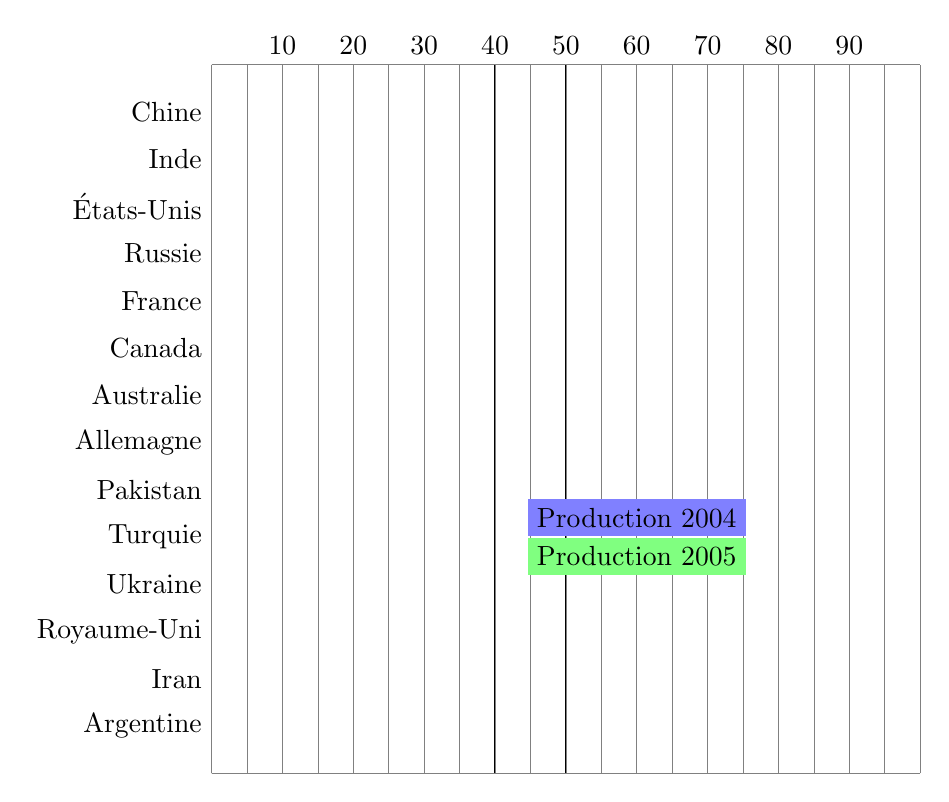
\begin{tikzpicture}[xscale=0.09, yscale=0.6]
		\draw (0,0) grid[xstep=10,ystep=15] (100,15);
		\draw[gray,very thin] (0,0) grid[xstep=5,ystep=15] (100,15);
		\draw[line width=4mm,color=blue!50]
		plot[xcomb] file {producBle2004.txt};
		
		\foreach \x in {10,20,...,90} \draw(\x,15)node[above]{\x};
		\foreach \n/\y in {Chine/14,Inde/13,États-Unis/12,Russie/11,
			France/10,Canada/9,Australie/8,Allemagne/7,Pakistan/6,
			Turquie/5,Ukraine/4,Royaume-Uni/3,Iran/2,Argentine/1}
		\draw (0,\y) node [left] {\n};
		
		\draw [line width=3mm,color=blue!50,yshift=2mm]
		plot[xcomb] file {producBle2004.txt};
		\draw [line width=3mm,color=green!50,yshift=-2mm]
		plot[xcomb] file {producBle2005.txt};
		
		\draw(60,5)node[fill=blue!50,above] {Production 2004};
		\draw(60,5)node[fill=green!50,below] {Production 2005};
		\end{tikzpicture}
	\end{center}
	
	\subsection{Courbe de variations de données}
	\subsubsection{Courbe des variations : \texttt{plot file}}
	% Problèmes des abscisses trop grandes pour Tikz, on fait donc du pré-traitement pour ramener les coordonnées dans une tranche raisonnable
	
	\begin{center}
		\begin{tikzpicture}
		\draw plot file {producRiz.txt};
		\end{tikzpicture}
	\end{center}

	\subsubsection{Quadrillage : \texttt{grid, step}}
	
	\begin{center}
		
\begin{tikzpicture}
		\draw (7,57) grid[ystep=5.00001mm] (16,64);
		\draw plot file {producRiz.txt};
		
		\end{tikzpicture}
	\end{center}

	\subsubsection{Annotations, décorations : \texttt{$\backslash$foreach, node, mark}}
	
	\begin{center}
		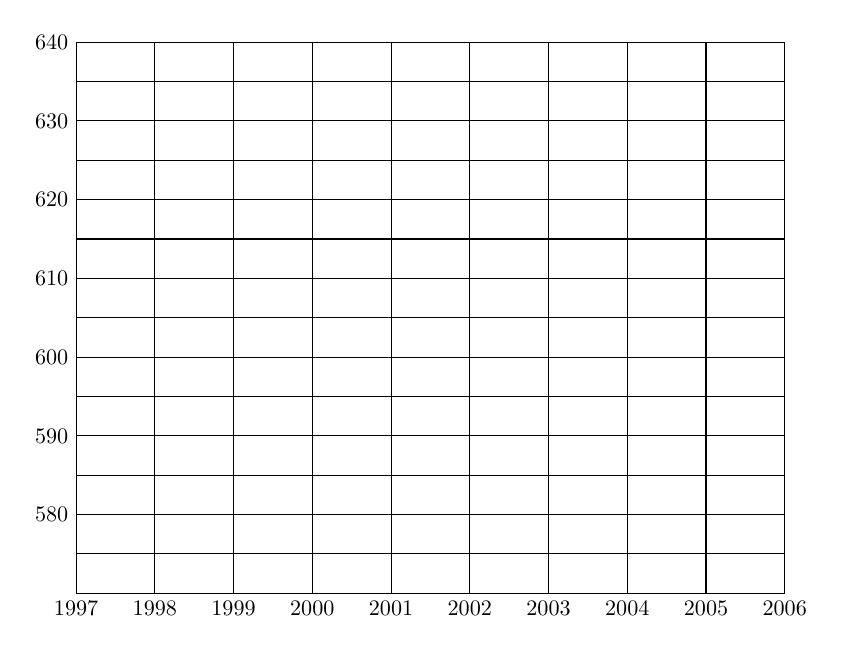
\begin{tikzpicture}
		\draw (7,57) grid[ystep=5.00001mm] (16,64);
		\draw plot[mark=ball,mark
		size=3pt] file {producRiz.txt};
		
		\foreach \y in {58,59,...,64}
		\draw (7,\y) node[left,scale=0.8]{\y0};
		\foreach \x in {1997,1998,...,2006}
		\draw (\x-1990,57) node [below,scale=0.8] {\x};
		\end{tikzpicture}
	\end{center}

	\subsection{Diagrammes à secteurs}
	
	\begin{center}
		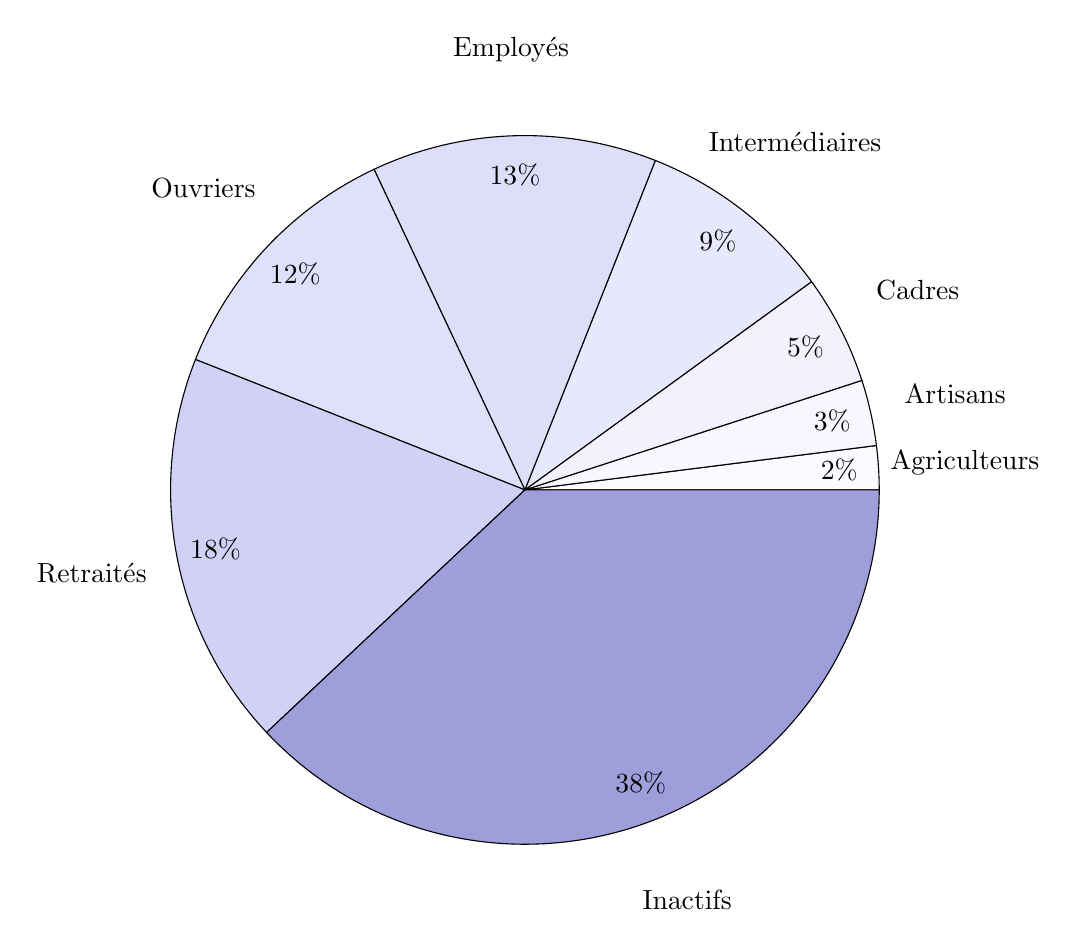
\begin{tikzpicture}
		\foreach \a/\b/\p/\c in
		{
			0/7.2/2/Agriculteurs, 7.2/18/3/Artisans,
			18/36/5/Cadres, 36/68.4/9/Intermédiaires,
			68.4/115.2/13/Employés, 115.2/158.4/12/Ouvriers,
			158.4/223.2/18/Retraités, 223.2/360/38/Inactifs
		}
		{
			\draw[fill=black!\p!blue!\p]
			(0,0) -- (\a:4.5) arc (\a:\b:4.5) -- cycle;
			\draw ({(\a+\b)/2}:4) node {\p\%};
			\draw ({(\a+\b)/2}:5.6) node {\c};
		}
		\end{tikzpicture}
	\end{center}
	
\section{Graphes : Introduction}
	\subsection{Voyelle ou consonne}
	
	\begin{center}
		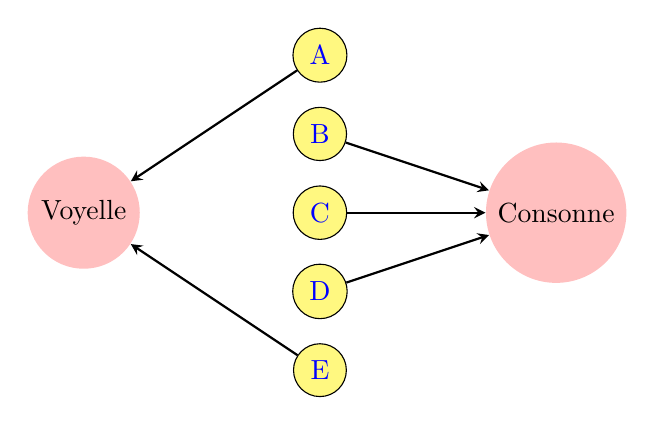
\begin{tikzpicture}
		\tikzstyle{lettre} = [circle,draw,fill=yellow!50,text=blue]
		\tikzstyle{type} = [circle,fill=red!25]
		\tikzstyle{fleche} = [->,>=stealth,thick]
		
		\node[lettre](A) at (0,2) {A};
		\node[lettre](B) at (0,1) {B};
		\node[lettre](C) at (0,0) {C};
		\node[lettre](D) at (0,-1) {D};
		\node[lettre](E) at (0,-2) {E};
		
		\node[type](Consonne) at (3,0) {Consonne};
		\node[type](Voyelle) at (-3,0) {Voyelle};
		
		\draw[fleche] (A) -- (Voyelle);
		\draw[fleche] (B) -- (Consonne);
		\draw[fleche] (C) -- (Consonne);
		\draw[fleche] (D) -- (Consonne);
		\draw[fleche] (E) -- (Voyelle);
		\end{tikzpicture}
	\end{center}
	
	\subsection{Les points cardinaux}
	
	\begin{center}
		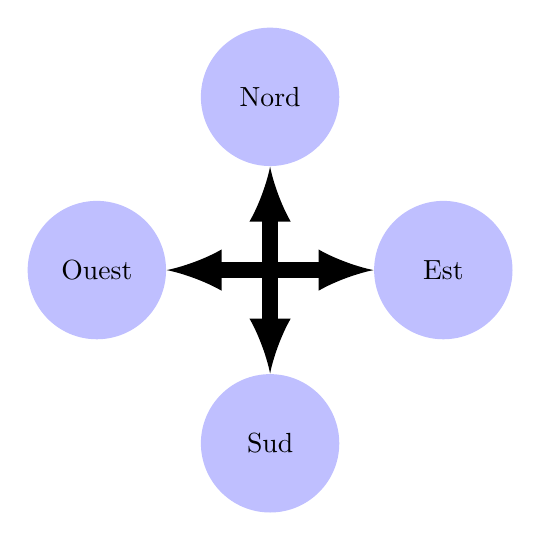
\begin{tikzpicture}[scale=1.1]
		\tikzstyle{point} = [circle,fill=blue!25,minimum width=5em]
		\tikzstyle{fleche} = [<->,>=latex,line width=2mm]
		
		\node[point](S) at (0,-2) {Sud};
		\node[point](N) at (0,2) {Nord};
		\node[point](E) at (2,0) {Est};
		\node[point](O) at (-2,0) {Ouest};
		
		\draw[fleche] (N) -- (S);
		\draw[fleche] (E) -- (O);
								
		
		\end{tikzpicture}
	\end{center}
	
	
\end{document}

